\documentclass[conference]{IEEEtran}
\IEEEoverridecommandlockouts
% The preceding line is only needed to identify funding in the first footnote. If that is unneeded, please comment it out.
%\usepackage{cite}
\usepackage{amsmath,amssymb,amsfonts}
\usepackage{algorithmic}
\usepackage{graphicx}
\usepackage{textcomp}
\usepackage{xcolor}
\usepackage{hyperref}
\usepackage{biblatex}
\usepackage{soul}
\usepackage{balance}
\usepackage{combelow}
\usepackage[normalem]{ulem}
\usepackage{multirow}
\addbibresource{bibliography.bib}

\def\BibTeX{{\rm B\kern-.05em{\sc i\kern-.025em b}\kern-.08em
    T\kern-.1667em\lower.7ex\hbox{E}\kern-.125emX}}
\begin{document}

\title{An Analysis of Multi-Task Architectures for the Hierarchic Multi-Label Problem of Vehicle Model and Make Classification}
% https://www.overleaf.com/project/625ad1dfab03cbf3da656f9b

\author{\IEEEauthorblockN{Alexandru Manole, Laura-Silvia Dio\cb{s}an}}

\author{
    \IEEEauthorblockN{Alexandru Manole\IEEEauthorrefmark{1} and Laura-Silvia Dio\c{s}an\IEEEauthorrefmark{1}}
    \IEEEauthorblockA{\IEEEauthorrefmark{1}Department of Computer Science, Babe\c{s}-Bolyai University, Cluj-Napoca, Romania \\
    \{alexandru.manole, laura.diosan\}@ubbcluj.ro}
}


\maketitle

\begin{abstract}
Most information in our world is organized hierarchically, however many Deep Learning approaches do not leverage this semantically rich structure. Research suggests that human learning benefits from capitalization on the hierarchical structure of information, and intelligent models could similarly exploit this through multi-task learning. In this work, we analyze the advantages and limitations of multi-task learning in a hierarchical multi-label classification problem: car make and model classification. Through extensive experiments, we measure its impact on different architectures (CNNs, Transformers) while varying key variables such as data augmentation, dropout, and loss weighting to gain deeper insights into the effectiveness of this approach.
\end{abstract}

\begin{IEEEkeywords}
Multitask Learning, Hierarchic Multi-Label Classification 
% Check their existance in IEEE Keywords
\end{IEEEkeywords}

\section{Introduction}
\label{sec:intro}

\IEEEPARstart{I}{n} the past decade Deep Learning approaches have been used successfully in numerous fields for a myriad of tasks. Usually, the training process focuses on a single task, in which the intelligent model becomes a specialist. Although this method can yield impressive performance, some limitations still restrict the performance of this technique. One such deficiency is related to the generalization capability of Deep Learning solutions, as the model can yield surprising and wrong predictions for out-of-distribution samples. 

In our world, many entities can be observed as part of a hierarchic structure. For example, a biologist order all discovered species using taxonomies with around 10 hierarchical levels, ranging from: \textit{Domain}, \textit{Kingdom} to \textit{Genus} and \textit{Species}. The stratified structure allows scientists to increase their understanding of each species. In addition to acting as a logical organizational form for specialists, hierarchical structures are considered an essential construction in the learning process, as shown by cognitive scientists \cite{botvinick2009hierarchically}, \cite{eckstein2021mind}, \cite{theves2021learning}. 

% annouce that we only deal with classification 

% add a figure to explain classification

Our hypothesis, which is also supported by innovative works in the literature \cite{chen2019deep}, \cite{pujari2021multi}, \cite{wang2021label},  \cite{wang2023consistency}, \cite{jiang2024hierarchical}, argues that deep learning model training benefits from the incorporation of additional information regarding the super-classes or sub-classes of the target classification task. These approaches apply a variety of techniques, in order to fully exploit the stratified label organization, including Multi-task Learning (\textbf{MTL}), a paradigm in which multiple objectives are combined in a single training procedure. MTL is a suitable choice for Hierarchic Multi-Label problems, as for each level from the taxonomy, a classification head can be created. 

Although multitask models are applied for hierarchic classification problems, the effects of the MTL architecture choice have yet to be thoroughly explored. Starting from the Vehicle Make and Model Classification (\textbf{VMMC}) problem, a challenge in which the intelligent system has to jointly predict the car make (i.e. 'Dacia') and model (i.e. 'Logan'), this paper investigates the behavior of MTL architectures. This work aims to provide answers to the following research questions. 

\begin{enumerate}
    \item[\textbf{RQ1}:] 
    How might the addition of cascaded and paralel MTL objectives influence the VMMC problem?
    \item[\textbf{RQ2}:] 
    How does the architecture of the base model (CNN, Transformer) influence the effectiveness of the multi-task model?
\end{enumerate}

The structure of the rest of this paper is the following: Section \ref{relWork} describes the related methods used for solving this task or other similar problems, Section \ref{sec:methodology} presents the proposed approach for the vehicle model and make classification task and Section \ref{results} describes the proposed experiments and the analysis of their results. The paper is concluded in Section \ref{conclusion}.

\section{Related Work}
\label{relWork}

\subsection{Multi-Task Learning}

Multi-Task is a Machine Learning paradigm introduced in \cite{caruana1997multitask} which aims to increase performance and generalization capabilities of intelligent models through the addition of symbiotic objectives. This model design philosophy proved itself useful in the deep learning era, achieving impressive results in both Computer Vision and Natural Language Processing \cite{zhang2021survey}. 

\begin{figure}[hbt!]
\centering
\centerline{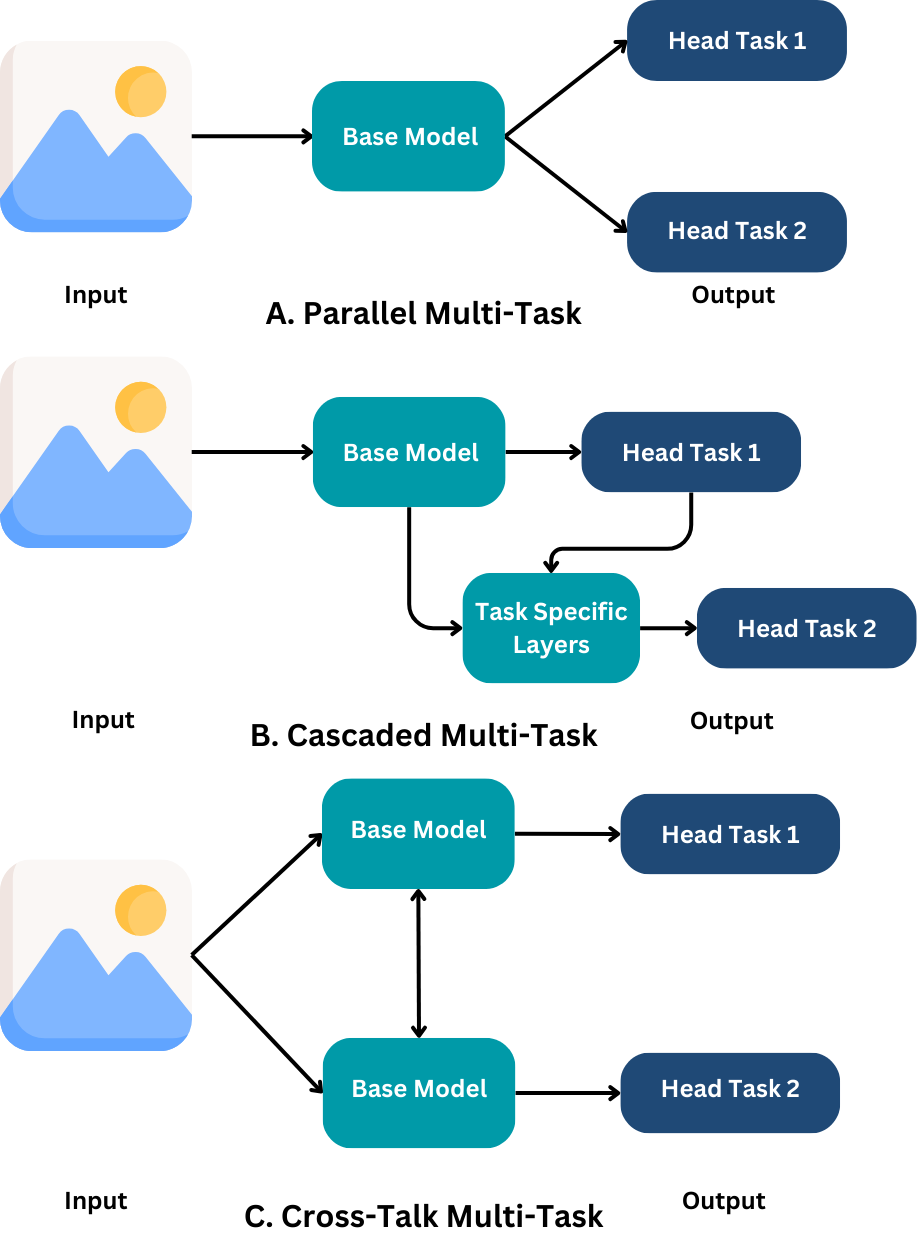
\includegraphics[scale=0.3]{figures/multi-task-taxonomy.png}}
	\caption{Simplified overview of multi-task architecures. (A) Parallel (B) Cascaded (C) Cross-Talk Multitask.}
	\label{fig:multi-task-taxonomy}
\end{figure}

Depending on the way the objectives and their features are combined, three main Multi-Task architectures exist: parallel, cascaded, and cross-talk. In the former, all tasks share the same encoder, which feeds its feature into task-specific layers for each classification objective. In the cascaded MTL, one of the tasks is solved initially, and some of the obtained features are used as part of the other tasks. The cross-talk architecture resembles the parallel one, the main difference being that in this structure two task-specific paths are allowed to communicate and share features through fusion modules. A simplified illustration of thee MTL architectures is present in \ref{fig:multi-task-taxonomy}.

\subsection{Hierarchic Multi-Label Classification}

\subsection{Vehicle Make and Model Classification}



Other approaches ... . Standford Cars \cite{krause2015fine}. CompCars \cite{yang2015large}

\section{Method}
\label{sec:methodology}

To fully exploit the hierarchic structure of datasets which offer multi-label stratified annotations in the form of super- and subclasses, we propose a multi-task approach. We start from three ubiquitous architectures: DenseNet121 \cite{huang2017densely}, MaxVit T \cite{tu2022maxvit}, and ConvNext Base \cite{liu2022convnet}. Our choice was based on two main factors. First of all, we wanted to measure the influence of MTL on different model families, thus we included a CNN and a Transformer model. ConvNext is a special case, as it is a modern CNN, which managed to achieve performances which rival transformer-based models by emulating some of their characteristics (i.e., increasing field-of-view, the usage of the inverted bottleneck). The second criterion used for the choice of base model was the performance obtained during an initial experiment on the Standford Cars dataset. This allowed us to select the most suitable model for this problem, from each category.  

Each model is explored in three forms. In the first one, the vanilla model is used as a baseline. The second and third add the multi-task architecture. The former introduces a parallel MTL objective, in the form of a classification head tasked with predicting the car's make. The latter adds the same output, but instead of the parallel structure a cascaded one is employed, thus the logits obtained from the car make classification are used as part of the decision and the more granular task of car model prediction. In \textbf{Table} \ref{tab:modealparameters}, we present the number of parameters of the base models and their parallel and cascaded multi-task variants.

\begin{table}[ht]
    \centering
    \scriptsize
    \caption{Number of parameters for each base and multi-task model.}
    \scalebox{1.2}{ 
    \begin{tabular}{||c c c||} 
     \hline
     \textbf{Model} & \textbf{No. Parameters} & \textbf{FLOPs}\\ 
     \hline\hline
     DenseNet-121 & 7,154,756 &  2,896,183,808 \\ 
     \hline
     DenseNet-121 Parallel & 7,204,981 & 2,896,233,984  \\
     \hline
     DenseNet-121 Cascaded & 7,214,585 & 2,896,243,588 \\
     \hline\hline
     MaxVit-T & 30,508,172 & 5,455,904,000 \\
     \hline
     MaxVit-T Parallel & 30,533,309 & 5,455,929,088 \\
     \hline
     MaxVit-T Cascaded & 30,542,913 & 5,455,938,692 \\
     \hline \hline
     ConvNext & 87,767,364 & 15,372,622,848 \\
     \hline
     ConvNext Parallel & 87,817,589 & 15,372,673,024 \\
     \hline
     ConvNext Cascaded & 87,827,193 & 15,372,682,628 \\ 
     \hline  
    \end{tabular}}
    \label{tab:modealparameters}
\end{table}

% TO DO: add citations to models
In addition to the model presented above, other established architectures were tested, including: MobileNet, ResNet, VGG, EfficientNet, Swin, and ViT. However, in our initial experiments with the Standford Cars dataset, they underperformed when compared to the three chosen base models by at least 5\% accuracy score. This trend continued even after the addition of the multi-task extensions. 

\section{Experiments}
\label{results}

\begin{figure*}[hbt!]
\centering
\centerline{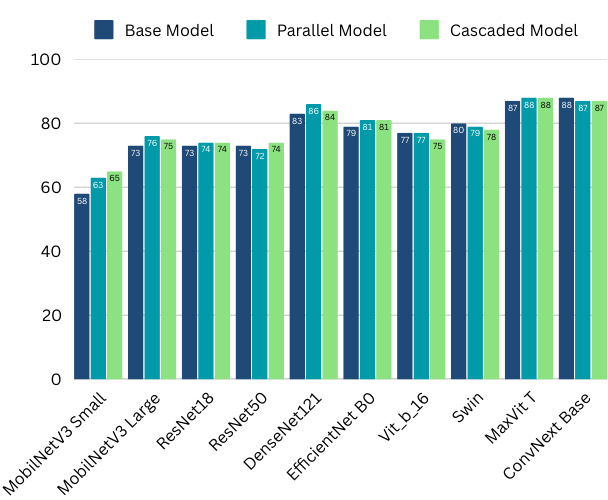
\includegraphics[scale=0.85]{figures/experiment0.png}}
	\caption{Test accuracy percentage for the initial experiment used for choosing the most promising base models.}
	\label{fig:experiment0}
\end{figure*}

In this section, we will provide additional information regarding our experimental setup including details about: the hardware, dataset characteristics, and hyper-parameters choices. 

\subsection{Dataset}

Standford Cars \cite{krause2015fine}, consists of 16,185 images split into two sets: 8,144 training samples and 8,041 testing samples. Each image contains a single car for which three labels are provided: the car's make, model, and year of fabrication. The samples have varying resolutions and most of the images being approximately 360 × 240 pixels. 

In the dataset, there are 196 classes for the model classification problem, which are part of 49 car-make classes. The distribution is balanced in both the training and the test sets. However, the test set labels are not publicly available. We conduct our experiments on the 8144 training samples, which we divide in three sets: training, validation, and test with the ratios 0.7, 0.2 and 0.1.  

% Add image of samples 

Standford Cars provides images captured in real scenes, with different angles and lightning conditions. These variables change even in the same class, resulting in a significant intra-class variation. Another challenge is the inter-class similarity as different models from the same manufactures can have similar shapes, especially from certain angles. Despite the difficulties, the hierarchic structure of the dataset and its "captured-in-the-wild" characteristics,  which reflect real-world, unconstrained conditions, make the dataset a desirable one for measuring the effects of multitask learning. 

\subsection{Results}

During our experiments, we resize the images to a resolution of 224x224. We train all models for 25 epochs, a value determined empirically which seems to be a point from which no further improvements are obtained with our algorithms. After our initial experiments, which used no augmentation, we employ the same set of transformations in order to add more variety to the relatively small training set of Standford Cars. This step has almost the same beneficial effect on all model configurations. To this end, we employ the Albumentation library \cite{buslaev2020albumentations} and construct a composed transformation consisting of random horizontal flips and changes to the brightness, contrast, saturation, and hue of an image. All have a random change of being applied, and the intensity of the change is set to be between certain values. 

The multi-task objective is optimized using Adam, starting from a learning rate of 3e-4 which is scheduled following the one-cycle \cite{smith2019super} policy. In this algorithm, the learning rate gradually increases from an initial value to a maximum value, followed by a gradual decrease, which becomes smaller than the initial learning rate value. 

In our investigation, a number of parameters vary from one experiment to another. Two of these variables are the loss weights used to balance the car model classification objective with the additional output of the car make prediction. Another important value which changes through our experiments is the dropout rate applied before the final prediction. It is interesting to observe the effects of the dropout and augmentation pipeline, especially when used in tandem with the MTL paradigm, as both have a regulative effect on the learning process. 

% Experiment 0 - Choice of three baselines

We introduced our variables step by step to carefully gauge the effect of the MTL architecture in isolation. Thus, the first experiment does not use augmentations or dropout layers, and the objective weights are set to 0.9 for the main task and 0.1 for the coarser secondary classification. The results obtained by the base models are depicted in \textbf{Figure} \ref{fig:experiment0}. We can observe that, from the list of examined models, DenseNet121 is the best suited foundational CNN for this task and dataset. When comparing the three transformer-based architectures \cite{vaswani2017attention}, MaxVit Tiny shows the highest potential. ConvNext also proves itself, again, as a powerful backbone which can rival any competing backbone. We decide to continue our experiments with both DenseNet and ConvNext as the latter introduces numerous changes to the architecture of traditional CNN in an effort to emulate the advantages of transformers. 

We continue by varying the weights that balance the importance of the two tasks. We choose 3 pairs of weights that cover the full spectrum: significantly more importance to the main task ([0.9, 0.1]), equal importance ([0.5, 0.5]), and more importance to make classification ([0.2, 0.8]). The results are shown in \textbf{Table } \ref{tab:experiment1}.

% Experiment 1 - Weights sum of 1 

\begin{table}[ht]
    \centering
    \scriptsize
    \caption{Test accuracy for car model prediction, no dropout and no augmentations.}
    \scalebox{1.25}{ 
    \begin{tabular}{||c c c c||} 
     \hline
     \textbf{Model} &  \textbf{Multi-Task} & \textbf{Loss Weights}  & \textbf{Acc.} \\
     \hline\hline
     DenseNet-121 & No & - & 0.833  \\ 
     \hline
     DenseNet-121 & Parallel & [0.9, 0.1] & \textbf{0.861} \\
     \hline
     DenseNet-121 & Cascaded & [0.9, 0.1] & 0.842 \\
     \hline
     DenseNet-121 & Parallel & [0.5, 0.5] & 0.833 \\
     \hline
     DenseNet-121 & Cascaded & [0.5, 0.5] & 0.826 \\
     \hline
     DenseNet-121 & Parallel & [0.2, 0.8] & 0.787  \\
     \hline
     DenseNet-121 & Cascaded & [0.2, 0.8] & 0.776\\
     \hline\hline
     MaxVit-T & No & - & 0.878 \\ 
     \hline
     MaxVit-T & Parallel & [0.9, 0.1] & \textbf{0.882}  \\
     \hline
     MaxVit-T & Cascaded & [0.9, 0.1] & 0.881 \\
     \hline
     MaxVit-T & Parallel & [0.5, 0.5] & 0.866  \\
     \hline
     MaxVit-T & Cascaded & [0.5, 0.5] & 0.864 \\
     \hline
     MaxVit-T & Parallel & [0.2, 0.8] & 0.871 \\
     \hline
     MaxVit-T & Cascaded & [0.2, 0.8] & 0.872 \\
     \hline \hline
     ConvNext & No & - & \textbf{0.883} \\ 
     \hline
     ConvNext & Parallel & [0.9, 0.1] & 0.873  \\
     \hline
     ConvNext & Cascaded & [0.9, 0.1] & 0.871 \\
     \hline
     ConvNext & Parallel & [0.5, 0.5] & 0.875  \\
     \hline
     ConvNext & Cascaded & [0.5, 0.5] & 0.861 \\
     \hline
     ConvNext & Parallel & [0.2, 0.8] & 0.842  \\
     \hline
     ConvNext & Cascaded & [0.2, 0.8] & 0.808 \\
     \hline  
    \end{tabular}}
    \label{tab:experiment1}
\end{table}

Certain trends become apparent when analysing the results. First, the parallel MTL usually outperforms the cascade variation. Secondly, as one might expect, as more importance is given to the model classification, the performance increases. A notable expectation is in the case of MaxVit-T where using weights favor the more course objective, the granular performance also increases, when compared to the prospect of using equal weights. Lastly, MTL yields better results when applied on DenseNet and MaxVit; however, based on the numerical results of the experiments, it seems to hinder the performance of ConvNext.

% Experiment 2 - Weights sum of 1 + dropout

As the previous experiment suggests, the use of the weights [0.9, 0.1] leads the MTL models to the best performance. An outlier is present in the form of the parallel ConvNext with equal weights, but since the difference is rather small and the MTL does not lead to the best performance in the model's case, we considered it acceptable to set the weights to the pair, which generally leads to better accuracy. In the next experiment, we introduced the dropout variable giving it three values: 0, 0.25 and 0.5. Although the experiments without dropout are equivalent to the ones from the previous table, we will also present them in \textbf{Table \ref{tab:experiment2}} to facilitate comparison.

\begin{table}[ht]
    \centering
    \scriptsize
    \caption{Test accuracy for car model prediction, weights (0.9, 0.1) and no augmentations.}
    \scalebox{1.25}{ 
    \begin{tabular}{||c c c c||} 
     \hline
     \textbf{Model} &  \textbf{Multi-Task} & \textbf{Dropout}  & \textbf{Acc.} \\
     \hline\hline
     DenseNet-121 & No & 0 & 0.833  \\ 
     \hline
     DenseNet-121 & Parallel & 0 & \textbf{0.861} \\
     \hline
     DenseNet-121 & Cascaded & 0 & 0.842 \\
     \hline
     DenseNet-121 & No & 0.25 & 0.832  \\ 
     \hline
     DenseNet-121 & Parallel & 0.25 & 0.841 \\
     \hline
     DenseNet-121 & Cascaded & 0.25& 0.835\\
     \hline
     DenseNet-121 & No & 0.5 & 0.832  \\ 
     \hline
     DenseNet-121 & Parallel & 0.5 & 0.844 \\
     \hline
     DenseNet-121 & Cascaded & 0.5 & 0.830 \\
     \hline\hline
     MaxVit-T& No & 0 & 0.878  \\ 
     \hline
     MaxVit-T & Parallel & 0 & \textbf{0.882} \\
     \hline
     MaxVit-T & Cascaded & 0 & 0.881 \\
     \hline
     MaxVit-T & No & 0.25 & 0.873  \\ 
     \hline
     MaxVit-T & Parallel & 0.25 & 0.864 \\
     \hline
     MaxVit-T & Cascaded & 0.25 & 0.877\\
     \hline
     MaxVit-T & No & 0.5 & 0.88  \\ 
     \hline
     MaxVit-T & Parallel & 0.5 & 0.869 \\
     \hline
     MaxVit-T & Cascaded & 0.5 & 0.873 \\
     \hline \hline
     ConvNext & No & 0 & 0.883  \\ 
     \hline
     ConvNext& Parallel & 0 & 0.873 \\
     \hline
     ConvNext& Cascaded & 0 & 0.871 \\
     \hline
     ConvNext& No & 0.25 & \textbf{0.894} \\ 
     \hline
     ConvNext& Parallel & 0.25 & 0.861 \\
     \hline
     ConvNext& Cascaded & 0.25& 0.862 \\
     \hline
     ConvNext& No & 0.5 & 0.866 \\ 
     \hline
     ConvNext& Parallel & 0.5 & 0.868 \\
     \hline
     ConvNext& Cascaded & 0.5 & 0.857 \\
     \hline  
    \end{tabular}}
    \label{tab:experiment2}
\end{table}

Combining MTL with dropout does not increase the performance of the models in the VMMC task. Looking at the full list of results, we can observe that parallel MTL with no dropout obtains the best results for DenseNet and MaxVit-T. The presence of a 0.25 dropout increases the accuracy of ConvNext, but this result is again without the additional objective. Another aspect which is worth mentioning is the fact that in the case of MaxVit-t with dropout the cascaded architecture obtains better results than the parallel one.

In our next experiments, we also focus on the accuracy results of the car-make classification problem. Moreover, we experiment again with the task weights, but this time we fix the main's objective importance to 1 and test different values for the car make weight (0.2, 0.5, 0.7).

% Experiment 3 - Weights + Dropout 

\newcommand{\multilinecell}[1]{%
    \begin{tabular}{@{}c@{}} #1 \end{tabular}%
}

% TO DO FIX CLASSIC ACCURACIES

% FLOPS +  NR PARAM -> NO. OP \ EPOCH
% TRAIN TIME FOR EACH TYPE OF MODEL

\begin{table}[ht]
    \centering
    \scriptsize
    \caption{Test accuracy for car model and make prediction, when online augmentation is used. In each accuracy cell, the first line showcases the performance of the normal non-multi-task method, while the second and third lines contain the accuracy for the parallel and cascaded MTL variants.}
    \scalebox{1.2}{ 
    \begin{tabular}{||c c c c c||} 
     \hline
     \textbf{Model} &  \textbf{\multilinecell{Loss \\ Weights}} & \textbf{Dropout}  & \textbf{\multilinecell{Model \\ Acc.}} & \textbf{\multilinecell{Make \\ Acc.}} \\
     \hline\hline
     DenseNet-121 & [1, 0.2] & 0.25 & \multilinecell{0.858 \\ \textbf{0.878} \\ 0.858} & \multilinecell{0.923 \\0.924\\ 0.908}\\
     \hline
     DenseNet-121 & [1, 0.5] & 0.25 & \multilinecell{0.858 \\ 0.869 \\ 0.859} & \multilinecell{0.923 \\\ \textbf{0.928} \\ 0.920}\\
     \hline
     DenseNet-121 & [1, 0.7] & 0.25 & \multilinecell{0.858 \\ 0.872 \\ 0.862} & \multilinecell{0.923 \\ \textbf{0.928} \\ 0.918}\\ 
     \hline
     DenseNet-121 & [1, 0.2] & 0.5 & \multilinecell{0.860 \\ 0.864 \\ 0.877} & \multilinecell{0.915 \\0.921\\ 0.921}\\   
     \hline
     DenseNet-121 & [1, 0.5] & 0.5 & \multilinecell{0.860 \\ 0.873 \\ 0.865} & \multilinecell{0.927 \\ \textbf{0.928} \\ 0.924}\\  
     \hline
     DenseNet-121 & [1, 0.7] & 0.5& \multilinecell{0.860 \\ 0.872 \\ 0.864} & \multilinecell{0.934 \\0.923\\ 0.916}\\  
     \hline \hline
     MaxVit-T & [1, 0.2] & 0.25 &\multilinecell{\textbf{0.895} \\ 0.893 \\ 0.887} & \multilinecell{0.949 \\ 0.950 \\ 0.938}\\  
     \hline
     MaxVit-T & [1, 0.5] & 0.25 & \multilinecell{\textbf{0.895}  \\ 0.894 \\ 0.887} & \multilinecell{0.949\\ 0.950 \\ 0.949}\\  
     \hline
     MaxVit-T & [1, 0.7] & 0.25 & \multilinecell{\textbf{0.895}  \\ 0.889 \\ 0.889 } & \multilinecell{0.949 \\ 0.950 \\ 0.943}\\  
     \hline
     MaxVit-T & [1, 0.2] & 0.5 & \multilinecell{0.892 \\ 0.891\\ 0.891} & \multilinecell{0.951 \\ 0.953\\ 0.936} \\ 
     \hline
     MaxVit-T & [1, 0.5] & 0.5 & \multilinecell{0.892 \\ 0.883 \\ 0.885 } & \multilinecell{0.951 \\0.945 \\ 0.947}\\  
     \hline
     MaxVit-T& [1, 0.7] & 0.5&  \multilinecell{0.892 \\ 0.894 \\ 0.865 } & \multilinecell{0.951 \\ \textbf{0.953} \\ 0.948}\\  
     \hline \hline
     ConvNext & [1, 0.2] & 0.25 & \multilinecell{\textbf{0.895} \\ 0.894 \\ 0.865 } & \multilinecell{0.952 \\ \textbf{0.953} \\ 0.948}\\   
     \hline
     ConvNext & [1, 0.5] & 0.25 & \multilinecell{\textbf{0.895} \\ 0.881 \\ 0.889 } & \multilinecell{0.952 \\0.933 \\ 0.938}\\ 
     \hline
     ConvNext & [1, 0.7] & 0.25 & \multilinecell{\textbf{0.895}\\ 0.883 \\ 0.888 } & \multilinecell{0.952 \\0.941\\ 0.945}\\ 
     \hline
     ConvNext & [1, 0.2] & 0.5 &  \multilinecell{0.886 \\0.861 \\ 0.861} &  \multilinecell{0.948 \\0.921 \\ 0.913} \\ 
     \hline
     ConvNext & [1, 0.5] & 0.5&  \multilinecell{0.886 \\ 0.888 \\ 0.879 } & \multilinecell{0.948 \\0.935 \\ 0.949}\\
     \hline
     ConvNext & [1, 0.7] & 0.5 & \multilinecell{0.886 \\ 0.889 \\ 0.877 } & \multilinecell{0.948 \\0.942 \\ 0.942}\\ 
     \hline \hline  
    \end{tabular}}
    \label{tab:experiment3}
\end{table}

Other trends emerge from the experiments presented in \textbf{Table} \ref{tab:experiment3}. The more coarse objective, car make classification, benefits from the prescience of the parallel MTL training procedure. As the base model only predicts the model of the car, we obtain the make by extracting the manufacturer from that prediction. As multitask architectures directly learn the make label, it is not surprising that it over-performs in this scenario. This is especially true for the DenseNet architecture. 

The use of augmentations makes both the base MaxVit-T and ConvNext achieve a top accuracy of 0.895. This is an improvement over the best performances obtained when no augmentations were present, especially for the transformer model. An MTL model derived from each MaxVit and ConvNext competes with the best performing base forms, achieving 0.894 accuracy, namely the parallel ConvNext with dropout 0.25, weighted [1, 0.2] and the parallel MaxVit with the same dropout with task weights [1, 0.5].

All of our experiments were conducted in the Google Colaboratory environment using the NVIDIA A100 Tensor Core GPU.  

\subsection{Discussion}


\begin{figure*}[hbt!]
\centering
\centerline{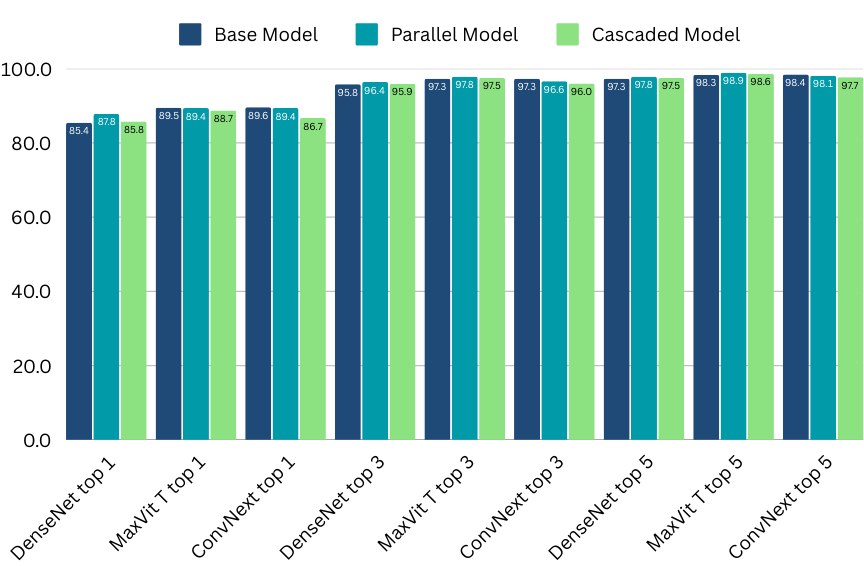
\includegraphics[scale=0.75]{figures/model_topn_accuracies.png}}
	\caption{Top 1, top 3 and top 5 model accuracies for DenseNet, MaxVit T and ConvNextBase in their base, parallel and cascaded form.   }
	\label{fig:topnaccuracies}
\end{figure*}


In \textbf{Fig.} \ref{fig:topnaccuracies} we showcase the performance of the best DenseNet, MaxVit and ConvNext obtained from all of our experiments. We go further than inspecting the pure performance and also analyse top 3 and top 5 accuracies. In ConvNext the same behavior is present through all metrics, namely the base models outperform the two MT variants. Similarly, for DenseNet the ranking of the top 1 accuracy remains unchanged for top 3 and top 5. In this model's case the additional multi-task objective is benefic, as both parallel and cascaded outperform the single-task variant. 

The most interesting development comes from the MaxVit T models. Even though the base model exceeds the performance of the cascaded and parallel ones in normal accuracy, for the other two metrics MT variants yield better results. Furthermore, the best top 5 accuracy is obtained by the parallel MaxVit T with a score of 98.9\% accuracy, better than DenseNet and ConvNext. This suggests that MTL embedded a broader semantic understanding, with potential to overperform when it comes to the recognition task in ambiguous cases, while maintaining an extremely competitive top 1 accuracy.


\begin{figure}[hbt!]
\centering
\centerline{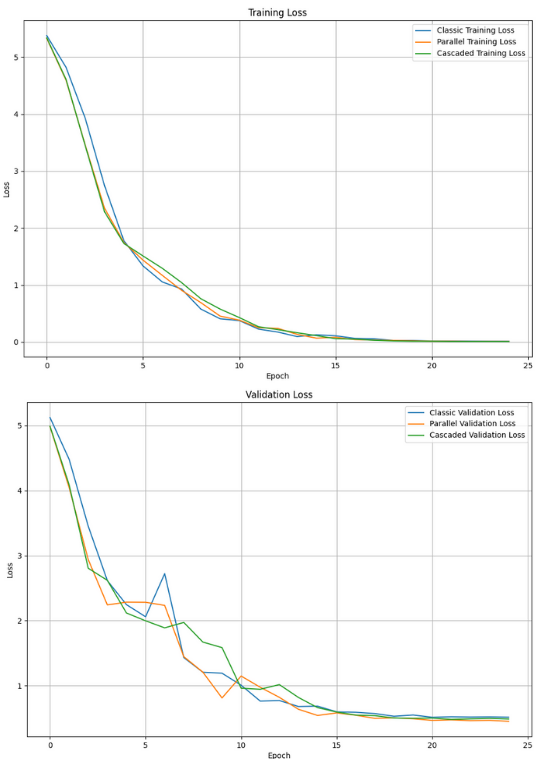
\includegraphics[scale=0.6]{figures/train_val_loss_densenet.png}}
	\caption{Evolution of train and validation loss values for classic, parallel and cascaded variants of DenseNet (with dropout 0.25 and loss weights [1, 0.2])}
	\label{fig:train_val_loss_densenet}
\end{figure}

In \textbf{Fig.} \ref{fig:train_val_loss_densenet}, the training and validation losses of the best DenseNet models are illustrated. Although the training accuracies are close together, being almost indistinguishable, for the validation test, which is not seen by the model, we can observe a different evolution. Models trained in the MTL formulation of the fine-grained car model classification problem have lower loss values for most of the learning process, especially the parallel variation. 

All of our results indicate that for this task, the addition of a second objective usually has a beneficial effect on the performance of the model, with a small cost, in terms of the number of parameters and FLOPs. Our CNN choice, DenseNet is the model which gains the most from this enhancement. For the investigated vision transformer, MaxVit T, the base and MT variants obtain almost the same top 1 accuracy score. In this scenario, the additional objectives aid in the secondary task (model recognition) and in top 5 accuracy, both suggesting a deep semantic understanding which could be less prone to overfitting. Lastly, ConvNext Base does not directly benefit from the proposed multi-task approach. We believe that this is not an illustration of the potential of symbiotic nature of this architecture and combined learning objective, but rather a manifestation of an incompatibility between a huge architecture and a small dataset. 

% Maybe answer to Research Question here for increased clarity 

\section{Conclusions and Future Considerations}
\label{conclusion}

In this work, we were able to showcase the benefits of the multi-task learning paradigm for a hierarchic multi-label problem, car model, and make classification. The advantages of this technique were illustrated for both the CNN and Transformer architectures. Furthermore, in the case of the former, the MTL architecture allows the relatively small DenseNet to rival larger and more modern architectures. 

Although we were able to showcase some of the advantages of the MTL approach, we strive to provide additional analysis in the future, in order to obtain a better understanding of this framework and its best uses. Thus, we identify the following future research direction: 
\begin{itemize}
    \item Extend the analysis by adding experiments with one or more types of cross-talk multi-task architectures
    \item Analyse the performance of parallel and cascaded models when the number of task-specific layers or blocks increases
    \item Conduct test on more datasets from this field or other hierarchic ones in order to extract a more general understanding of the behaviour of MTL models
    \item Experiment and analyse the behaviour of parallel, cascaded and cross-talk multi-task and tasks different than classification, including, but not limited to semantic segmentation and detection.
\end{itemize}



\balance


\printbibliography

\vfill

\end{document}